\documentclass[spanish]{article}

\usepackage{arxiv}

\usepackage[utf8]{inputenc} % allow utf-8 input
\usepackage[T1]{fontenc}    % use 8-bit T1 fonts
\usepackage{lmodern}        % https://github.com/rstudio/rticles/issues/343
\usepackage{hyperref}       % hyperlinks
\usepackage{url}            % simple URL typesetting
\usepackage{booktabs}       % professional-quality tables
\usepackage{amsfonts}       % blackboard math symbols
\usepackage{nicefrac}       % compact symbols for 1/2, etc.
\usepackage{microtype}      % microtypography
\usepackage{graphicx}
\usepackage[backend=biber, style=apa, language=spanish]{biblatex}
\addbibresource{references.bib}
\usepackage{csquotes}
\usepackage[rgb,html,cmyk]{xcolor}


\title{TÍTULO EN ESPAÑOL \newline \textit{\large TÍTULO EN INGLÉS}}

\author{
    \parbox[t]{10cm}{\centering NOMBRE1-NOMBRE2 APELLIDO1-APELLIDO2 \\ \orcidlink{CÓDIGO ORCID}}
   \\
    Universidad Autónoma de Santo Domingo (UASD) \\
  Santo Domingo, República Dominicana \\
  \texttt{\href{mailto:ESTUDIANTE@SERVIDOR.COM}{\nolinkurl{ESTUDIANTE@SERVIDOR.COM}}} \\
  }

% Pandoc syntax highlighting
\usepackage{color}
\usepackage{fancyvrb}
\newcommand{\VerbBar}{|}
\newcommand{\VERB}{\Verb[commandchars=\\\{\}]}
\DefineVerbatimEnvironment{Highlighting}{Verbatim}{commandchars=\\\{\}}
% Add ',fontsize=\small' for more characters per line
\usepackage{framed}
\definecolor{shadecolor}{RGB}{248,248,248}
\newenvironment{Shaded}{\begin{snugshade}}{\end{snugshade}}
\newcommand{\AlertTok}[1]{\textcolor[rgb]{0.94,0.16,0.16}{#1}}
\newcommand{\AnnotationTok}[1]{\textcolor[rgb]{0.56,0.35,0.01}{\textbf{\textit{#1}}}}
\newcommand{\AttributeTok}[1]{\textcolor[rgb]{0.13,0.29,0.53}{#1}}
\newcommand{\BaseNTok}[1]{\textcolor[rgb]{0.00,0.00,0.81}{#1}}
\newcommand{\BuiltInTok}[1]{#1}
\newcommand{\CharTok}[1]{\textcolor[rgb]{0.31,0.60,0.02}{#1}}
\newcommand{\CommentTok}[1]{\textcolor[rgb]{0.56,0.35,0.01}{\textit{#1}}}
\newcommand{\CommentVarTok}[1]{\textcolor[rgb]{0.56,0.35,0.01}{\textbf{\textit{#1}}}}
\newcommand{\ConstantTok}[1]{\textcolor[rgb]{0.56,0.35,0.01}{#1}}
\newcommand{\ControlFlowTok}[1]{\textcolor[rgb]{0.13,0.29,0.53}{\textbf{#1}}}
\newcommand{\DataTypeTok}[1]{\textcolor[rgb]{0.13,0.29,0.53}{#1}}
\newcommand{\DecValTok}[1]{\textcolor[rgb]{0.00,0.00,0.81}{#1}}
\newcommand{\DocumentationTok}[1]{\textcolor[rgb]{0.56,0.35,0.01}{\textbf{\textit{#1}}}}
\newcommand{\ErrorTok}[1]{\textcolor[rgb]{0.64,0.00,0.00}{\textbf{#1}}}
\newcommand{\ExtensionTok}[1]{#1}
\newcommand{\FloatTok}[1]{\textcolor[rgb]{0.00,0.00,0.81}{#1}}
\newcommand{\FunctionTok}[1]{\textcolor[rgb]{0.13,0.29,0.53}{\textbf{#1}}}
\newcommand{\ImportTok}[1]{#1}
\newcommand{\InformationTok}[1]{\textcolor[rgb]{0.56,0.35,0.01}{\textbf{\textit{#1}}}}
\newcommand{\KeywordTok}[1]{\textcolor[rgb]{0.13,0.29,0.53}{\textbf{#1}}}
\newcommand{\NormalTok}[1]{#1}
\newcommand{\OperatorTok}[1]{\textcolor[rgb]{0.81,0.36,0.00}{\textbf{#1}}}
\newcommand{\OtherTok}[1]{\textcolor[rgb]{0.56,0.35,0.01}{#1}}
\newcommand{\PreprocessorTok}[1]{\textcolor[rgb]{0.56,0.35,0.01}{\textit{#1}}}
\newcommand{\RegionMarkerTok}[1]{#1}
\newcommand{\SpecialCharTok}[1]{\textcolor[rgb]{0.81,0.36,0.00}{\textbf{#1}}}
\newcommand{\SpecialStringTok}[1]{\textcolor[rgb]{0.31,0.60,0.02}{#1}}
\newcommand{\StringTok}[1]{\textcolor[rgb]{0.31,0.60,0.02}{#1}}
\newcommand{\VariableTok}[1]{\textcolor[rgb]{0.00,0.00,0.00}{#1}}
\newcommand{\VerbatimStringTok}[1]{\textcolor[rgb]{0.31,0.60,0.02}{#1}}
\newcommand{\WarningTok}[1]{\textcolor[rgb]{0.56,0.35,0.01}{\textbf{\textit{#1}}}}

% tightlist command for lists without linebreak
\providecommand{\tightlist}{%
  \setlength{\itemsep}{0pt}\setlength{\parskip}{0pt}}

% From pandoc table feature
\usepackage{longtable,booktabs,array}
\usepackage{calc} % for calculating minipage widths
% Correct order of tables after \paragraph or \subparagraph
\usepackage{etoolbox}
\makeatletter
\patchcmd\longtable{\par}{\if@noskipsec\mbox{}\fi\par}{}{}
\makeatother
% Allow footnotes in longtable head/foot
\IfFileExists{footnotehyper.sty}{\usepackage{footnotehyper}}{\usepackage{footnote}}
\makesavenoteenv{longtable}


\usepackage{orcidlink} \usepackage{float} \usepackage[all]{nowidow} \usepackage[spanish]{babel} \usepackage{pdflscape} \renewcommand\spanishtablename{Tabla} \usepackage{xcolor} \usepackage{tabu} \renewcommand\tablename{Tabla} \renewcommand\figurename{Figura} \usepackage{xurl} \usepackage{fancyvrb} \usepackage[left]{lineno} \linenumbers
\usepackage{booktabs}
\usepackage{longtable}
\usepackage{array}
\usepackage{multirow}
\usepackage{wrapfig}
\usepackage{float}
\usepackage{colortbl}
\usepackage{pdflscape}
\usepackage{tabu}
\usepackage{threeparttable}
\usepackage{threeparttablex}
\usepackage[normalem]{ulem}
\usepackage{makecell}
\usepackage{xcolor}
\begin{document}
\maketitle


\begin{resumen}
RESUMEN EN ESPAÑOL. NO INTRODUCIR RETORNOS
\end{resumen}

\palabrasclave{
    PALABRA CLAVE EN ESPAÑOL
   \and
    PALABRA CLAVE EN ESPAÑOL
   \and
    PALABRA CLAVE EN ESPAÑOL
   \and
    PALABRA CLAVE EN ESPAÑOL
  }

%\newpage

\begin{abstract}
RESUMEN EN INGLÉS. NO INTRODUCIR RETORNOS
\end{abstract}

\keywords{
    PALABRA CLAVE EN INGLÉS
   \and
    PALABRA CLAVE EN INGLÉS
   \and
    PALABRA CLAVE EN INGLÉS
   \and
    PALABRA CLAVE EN INGLÉS
  }

\begin{quote}
Nota 1 del Tali: el uso de MAYÚSCULAS en esta plantilla, no significa
``estoy gritando'', sino una convención para indicarte dónde debes
rellenar contenido. Tan pronto leas el mensaje escrito en mayúsculas,
bórralo para que no quede en tu entrega.
\end{quote}

\begin{quote}
Nota 2 del Tali: pide ayuda a inteligencia artificial, y recuerda
también usar el foro en caso de ``tranque''.
\end{quote}

\section{Introducción}\label{introducciuxf3n}

\begin{itemize}
\item
  ESCRIBE AQUÍ LA SECCIÓN ``INTRODUCCIÓN''.
\item
  INCLUYE REFERENCIAS BIBLIOGRÁFICAS. LA SECCIÓN ``INTRODUCCIÓN'' ES UN
  BUEN LUGAR PARA ELLO. PARA CITAS DIRECTAS, USA
  \textcite{ETIQUETA_BIBTEX}. INCLUYE LA CITA ENTRE CORCHETES,
  \autocite{ETIQUETA_BIBTEX}, SI QUIERES QUE, EN EL PDF TEJIDO, LA CITA
  APAREZCA ``(AUTOR, AÑO)''.
\item
  INSERTA AQUÍ UNA FIGURA DE ARCHIVO (E.G. UN ÚNICO ARCHIVO, SÓLO UNO,
  QUE MUESTRE, AUNQUE SEA PARCIALMENTE, LO QUE ENTREGASTE EN LA PRÁCTICA
  02. SI NO TIENES DICHO ARCHIVO, PUEDES USAR CUALQUIER OTRO ARCHIVO
  ALEGÓRICO AL TEMA O A LA PRÁCTICA).
\end{itemize}

\section{Materiales y métodos}\label{materiales-y-muxe9todos}

\begin{itemize}
\item
  ESCRIBE AQUÍ LA SECCIÓN ``MATERIALES Y MÉTODOS''.
\item
  INCLUYE REFERENCIAS BIBLIOGRÁFICAS. LA SECCIÓN ``MATERIALES Y
  MÉTODOS'' ES TAMBIÉN UN BUEN LUGAR PARA ELLO. PARA CITAS DIRECTAS, USA
  \textcite{ETIQUETA_BIBTEX}. INCLUYE LA CITA ENTRE CORCHETES,
  \autocite{ETIQUETA_BIBTEX}, SI QUIERES QUE, EN EL PDF TEJIDO, LA CITA
  APAREZCA ``(AUTOR, AÑO)''.
\item
  INSERTA FIGURAS, COMO MAPAS DE LOCALIZACIÓN O MOSTRANDO TU DEM.
\item
  INCLUYE AQUÍ TABLAS DE DATOS DE FORMA ESTILIZADA, USANDO CÓDIGO DE R
  REPRODUCIBLE, COMANDO \texttt{knitr::kable} o
  \texttt{kableExtra::kable}, O DIRECTAMENTE EN MARKDOWN.
\end{itemize}

\section{Resultados}\label{resultados}

\begin{itemize}
\item
  ESCRIBE AQUÍ LA SECCIÓN ``RESULTADOS''.
\item
  INSERTA FIGURAS, TABLAS GENERADAS CON \texttt{knitr::kable} o
  \texttt{kableExtra::kable}, O DIRECTAMENTE EN MARKDOWN.
\item
  NO INSERTES RESULTADOS DE ANÁLISIS ESTADÍSTICOS TAL CUAL (POR EJEMPLO,
  NO PONGAS UNA CAPTURA DE PANTALLA DE R); LOS RESULTADOS DE ANÁLISIS
  ESTADÍSTICOS SE PRESENTAN COMO REDACCIÓN FLUIDA, O SI SON MUY DENSOS,
  EN FORMA DE TABLAS O GRÁFICOS.
\end{itemize}

\section{Discusión}\label{discusiuxf3n}

\begin{itemize}
\item
  ESCRIBE AQUÍ LA SECCIÓN ``DISCUSIÓN''.
\item
  SI LO DESEAS, INCLUYE AQUÍ REFERENCIAS BIBLIOGRÁFICAS. LA SECCIÓN
  ``DISCUSIÓN'' ES TAMBIÉN UN BUEN LUGAR PARA ELLO. PARA CITAS DIRECTAS,
  USA \textcite{ETIQUETA_BIBTEX}. INCLUYE LA CITA ENTRE CORCHETES,
  \autocite{ETIQUETA_BIBTEX}, SI QUIERES QUE, EN EL PDF TEJIDO, LA CITA
  APAREZCA ``(AUTOR, AÑO)''.
\end{itemize}

\section{Nota sobre las referencias cruzadas (ELIMINA ESTA SECCIÓN
CUANDO HAYAS GENERADO TU
DOCUMENTO)}\label{nota-sobre-las-referencias-cruzadas-elimina-esta-secciuxf3n-cuando-hayas-generado-tu-documento}

\subsection{\texorpdfstring{Poner título y usar referencias cruzadas
para tablas generadas con
\texttt{kableExtra}}{Poner título y usar referencias cruzadas para tablas generadas con kableExtra}}\label{poner-tuxedtulo-y-usar-referencias-cruzadas-para-tablas-generadas-con-kableextra}

El bloque de código debería comenzar con
\texttt{\{r\ tablaejemplokable,\ echo=FALSE\}}, donde
\texttt{\{r\ tablaejemplokable\}} sería la etiqueta para hacer la
referencia cruzada. Nota que se debería usar también
\texttt{echo=FALSE}, para que el código no se imprima, y sólo salga la
tabla tras el tejido. Así se vería el código y la tabla saldría justo
después:

\begin{Shaded}
\begin{Highlighting}[]
\FunctionTok{library}\NormalTok{(tidyverse)}
\FunctionTok{library}\NormalTok{(kableExtra)}
\FunctionTok{kable}\NormalTok{(}
  \AttributeTok{x =}\NormalTok{ mtcars[}\DecValTok{1}\SpecialCharTok{:}\DecValTok{5}\NormalTok{, }\DecValTok{1}\SpecialCharTok{:}\DecValTok{5}\NormalTok{],}
  \AttributeTok{caption =} \StringTok{"Título de la tabla de ejemplo generada con kableExtra"}\NormalTok{,}
  \AttributeTok{booktabs =} \ConstantTok{TRUE}\NormalTok{) }\SpecialCharTok{\%\textgreater{}\%}
  \FunctionTok{kable\_styling}\NormalTok{(}\AttributeTok{latex\_options =} \StringTok{"HOLD\_position"}\NormalTok{) }\SpecialCharTok{\%\textgreater{}\%}
  \FunctionTok{footnote}\NormalTok{(}\AttributeTok{general =} \StringTok{"Esta es una nota de una tabla generada con kableExtra."}\NormalTok{)}
\end{Highlighting}
\end{Shaded}

\begin{table}[H]
\centering
\caption{\label{tab:tablaejemplokable}Título de la tabla de ejemplo generada con kableExtra}
\centering
\begin{tabular}[t]{lrrrrr}
\toprule
  & mpg & cyl & disp & hp & drat\\
\midrule
Mazda RX4 & 21.0 & 6 & 160 & 110 & 3.90\\
Mazda RX4 Wag & 21.0 & 6 & 160 & 110 & 3.90\\
Datsun 710 & 22.8 & 4 & 108 & 93 & 3.85\\
Hornet 4 Drive & 21.4 & 6 & 258 & 110 & 3.08\\
Hornet Sportabout & 18.7 & 8 & 360 & 175 & 3.15\\
\bottomrule
\multicolumn{6}{l}{\rule{0pt}{1em}\textit{Note: }}\\
\multicolumn{6}{l}{\rule{0pt}{1em}Esta es una nota de una tabla generada con kableExtra.}\\
\end{tabular}
\end{table}

La referencia cruzada se debe escribir así ``Ver tabla
\texttt{\textbackslash{}ref\{tab:tablaejemplokable\}}'', y cuando el
documento se teja, quedaría algo tal que esto ``Ver tabla
\ref{tab:tablaejemplokable}''.

\subsection{Poner título y usar referencias cruzadas para tablas
generadas manualmente usando sintaxis
Markdown}\label{poner-tuxedtulo-y-usar-referencias-cruzadas-para-tablas-generadas-manualmente-usando-sintaxis-markdown}

La tabla que usa la sintaxis Markdown se escribe como se muestra abajo.
Nota que el título está justo debajo, precedido de la palabra clave con
dos puntos \texttt{Table:} y, al final aparece
``\texttt{\textbackslash{}label}'':

\begin{Verbatim}[samepage=true]
| Columna 1 | Columna 2 | Columna 3 |
|-----------|------------|-----------|
| dato 1    | dato 2     | dato 3    |
| dato 4    | dato 5     | dato 6    |
Table:Título de la tabla de ejemplo generada manualmente.\label{tab:tablaejemplomanualmente}
\end{Verbatim}

Una vez tejido el documento, la referencia se vería así ``Ver tabla
\ref{tab:tablaejemplomanualmente}'', y la tabla se representaría así con
su correspondiente título:

\begin{longtable}[]{@{}lll@{}}
\caption{Título de la tabla de ejemplo generada
manualmente.\label{tab:tablaejemplomanualmente}}\tabularnewline
\toprule\noalign{}
Columna 1 & Columna 2 & Columna 3 \\
\midrule\noalign{}
\endfirsthead
\toprule\noalign{}
Columna 1 & Columna 2 & Columna 3 \\
\midrule\noalign{}
\endhead
\bottomrule\noalign{}
\endlastfoot
dato 1 & dato 2 & dato 3 \\
dato 4 & dato 5 & dato 6 \\
\end{longtable}

\subsection{Poner título y usar referencias cruzadas para figuras
insertadas
manualmente}\label{poner-tuxedtulo-y-usar-referencias-cruzadas-para-figuras-insertadas-manualmente}

Para insertar una figura manualmente (el archivo debe estar disponible
en la ruta donde es llamado, en este caso, en el directorio raíz del
repo), es necesario hacero usando la sintaxis apropiada mostrada abajo
(nota que apliqué un redimensionamiento a 35\%, pero no es obligatorio).

\begin{Verbatim}[samepage=true]
![Una figura de ejemplo insertada manualmente](figura-ejemplo.jpg){width=25%,height=25%}
\label{fig:figuramanual}
\end{Verbatim}

La sintaxis para insertar la referencia cruzada sería ésta:
\texttt{Ver\ Fig.\ \textbackslash{}ref\{fig:figuramanual\}}.

Luego del tejido, la referencia cruzada se vería así ``Ver Fig.
\ref{fig:figuramanual}'' y la figura propiamiente se vería así:

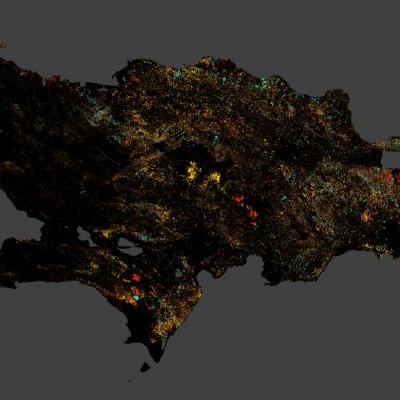
\includegraphics{figura-ejemplo.jpg} \label{fig:figuramanual}

\subsection{Poner título y usar referencias cruzadas para figuras
insertadas a partir de código de
R}\label{poner-tuxedtulo-y-usar-referencias-cruzadas-para-figuras-insertadas-a-partir-de-cuxf3digo-de-r}

El bloque de código debería comenzar con
\texttt{\{r\ figuraconcodigo,\ fig.cap="Esta\ es\ una\ figura\ generada\ con\ código",\ fig.width=0.5,\ fig.align=\textquotesingle{}center\textquotesingle{},\ echo=FALSE,\ fig.pos=\textquotesingle{}!H\textquotesingle{}\}},
donde la primer parte \texttt{\{r\ figuraconcodigo\}} sería la etiqueta
para hacer la referencia cruzada. Nota que se debería usar también
\texttt{echo=FALSE}, para que el código no se imprima, y sólo salga la
figura tras el tejido, y para que quede en posición, se usa
\texttt{fig.pos=\textquotesingle{}!H\textquotesingle{}}. También se usa
\texttt{fig.cap=""} para definir el título de la figura, y otras
opciones adicionales. Así se debería escribir el código y la figura
saldría justo después:

\begin{Shaded}
\begin{Highlighting}[]
\FunctionTok{plot}\NormalTok{(cars)}
\end{Highlighting}
\end{Shaded}

\begin{figure}[H]

{\centering 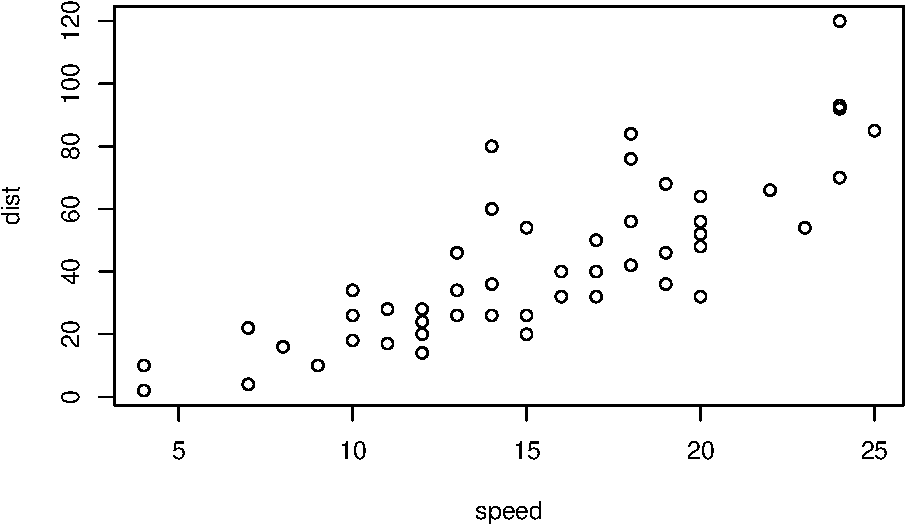
\includegraphics[width=0.5\linewidth]{manuscrito_files/figure-latex/figuraconcodigo-1} 

}

\caption{Esta es una figura generada con código}\label{fig:figuraconcodigo}
\end{figure}

La referencia cruzada se debe escribir así ``Ver Fig.
\texttt{\textbackslash{}ref\{fig:figuraconcodigo\}}'', y cuando el
documento se teja, quedaría algo tal que esto ``Ver Fig.
\ref{fig:figuraconcodigo}''.

\printbibliography


\end{document}
